\subsection{Private Aggregation of Teacher Ensembles}\label{sec:pate}

Die Private Aggregation of Teacher Ensembles Architektur (kurz PATE-Architektur) wurde 2017 von Papernot et al. \cite{P-57} erstmals vorgestellt.
Dabei handelt es sich um eine sogenannte Wissenstransfer-Architektur (Knowledge Transfer), bei welcher mindesten ein Modell genutzt wird, um ein weiteres Modell zu trainieren.

\begin{figure}[!htb]
    \centering
    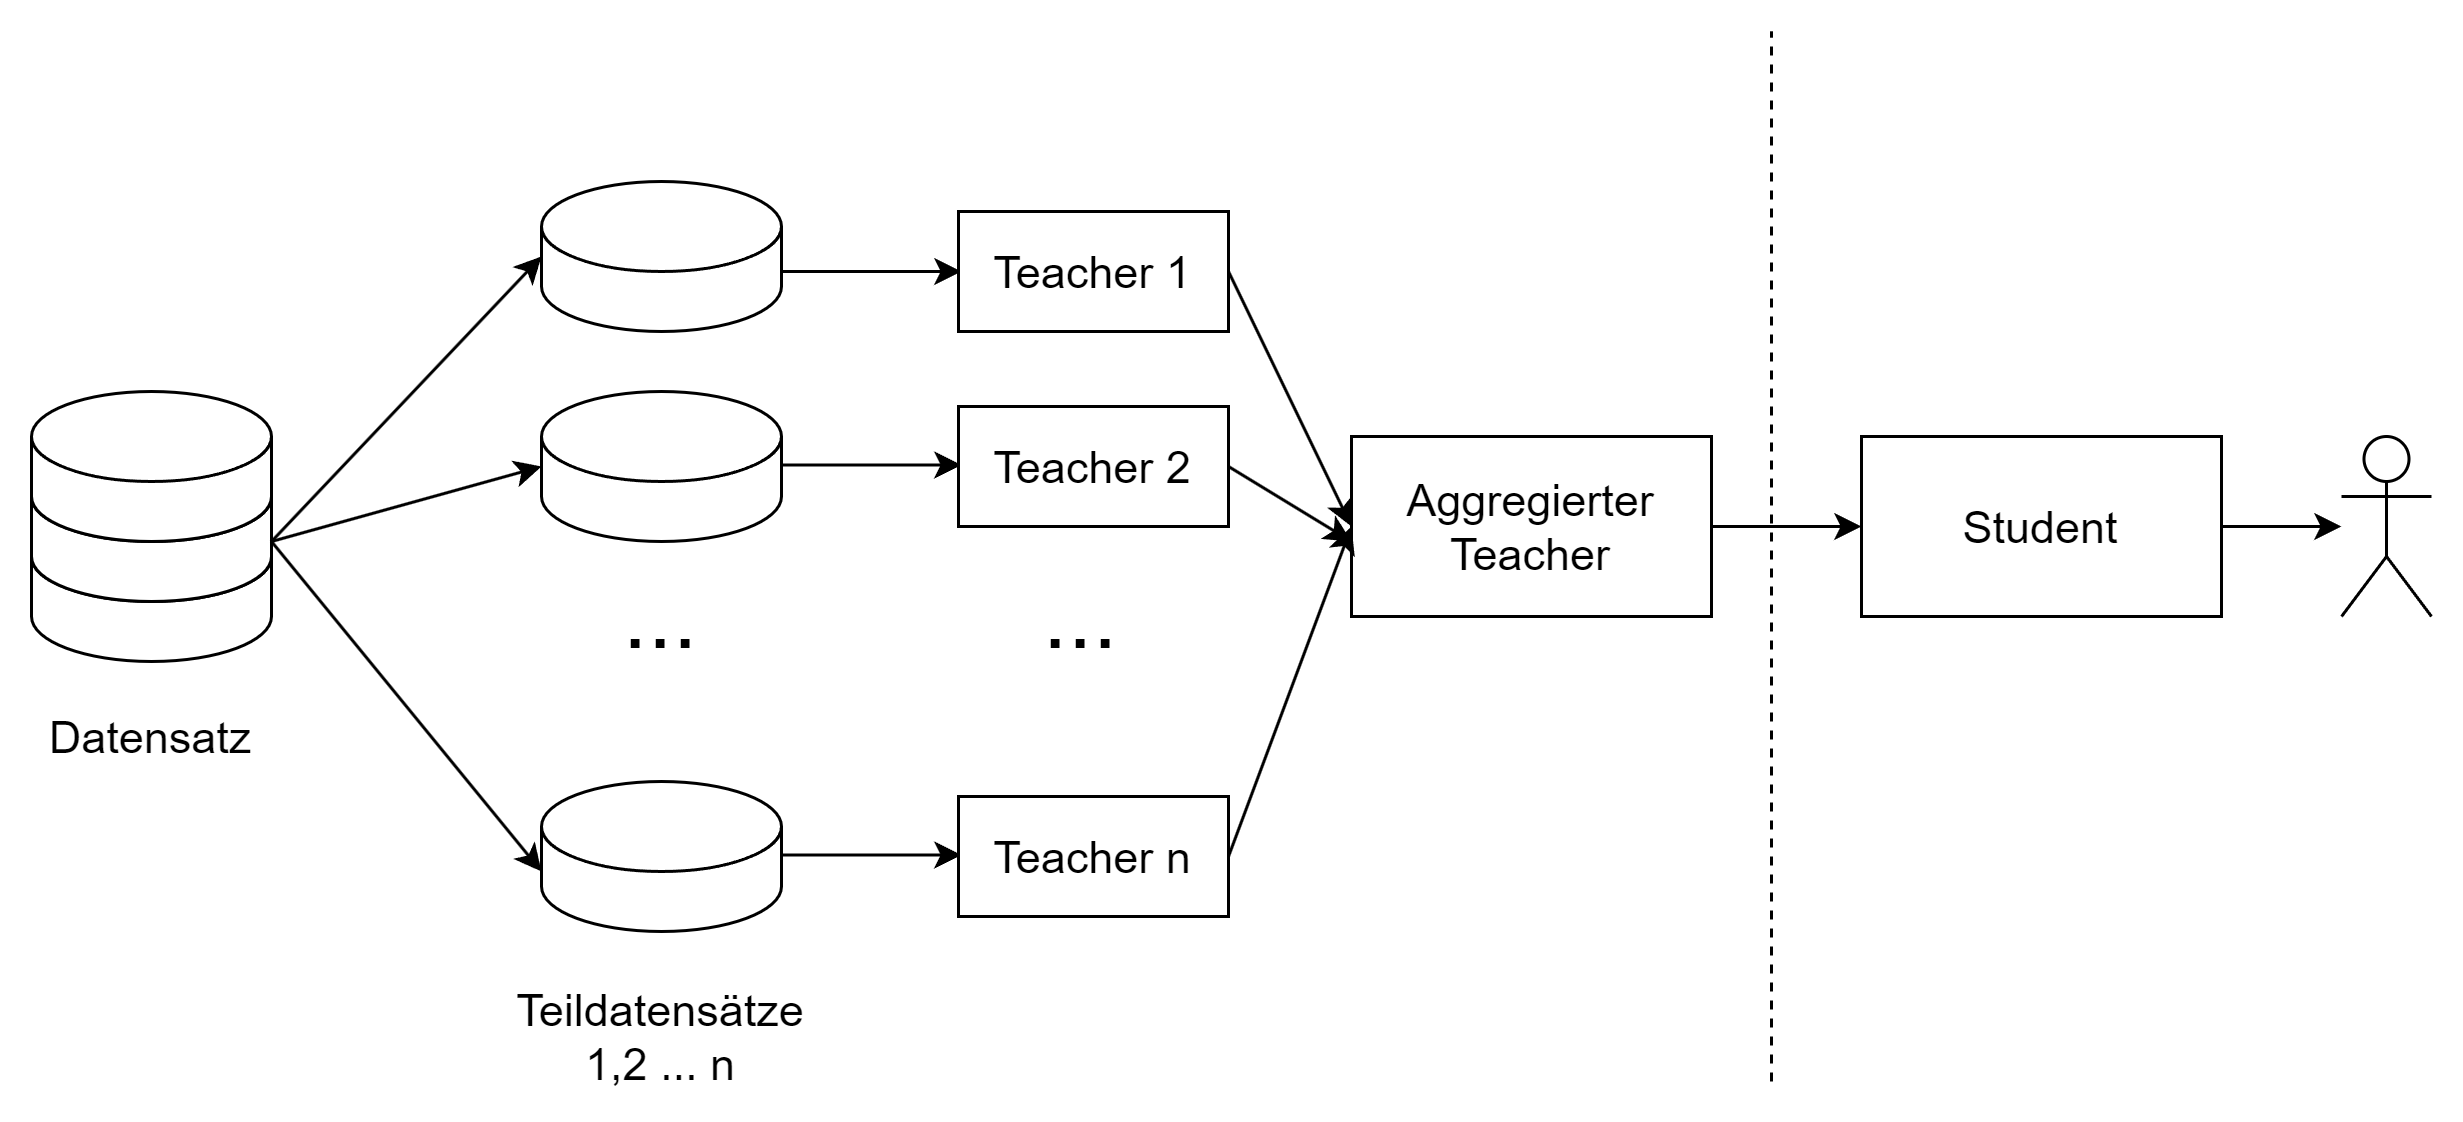
\includegraphics[width=15cm]{figures/pate_basic.png}
    \caption{PATE-Architektur nach \cite{P-57}}
    \label{fig:pate_basic}
\end{figure} 

Abbildung \ref{fig:pate_basic} zeigt eine Übersicht der PATE-Architektur.
Der Datenbestand wird dabei zuerst in verschiedene Teildatenmengen aufgeteilt. 
Für jede dieser Teildatenmengen wird anschließend ein sogenanntes Teacher oder Lehrer-Modell trainiert.
Wenn das gesamte Modell eine Klassifikation aus 10 unterschiedlichen Klassen vornimmt, dann muss jedes Teacher-Modell ebenfalls genau diese 10 Klassen abbilden.
Die Teacher-Modelle müssen also die gleiche Aufgabe bewältigen, wie das gesamte Modell.
Hierbei ist es ebenfalls wichtig, dass die Teildatenmengen nicht zu klein sind, da ansonsten die Teacher-Modelle nicht gut funktionieren würden.

Die Teacher-Modelle werden anschließend genutzt, um einen Trainingsdatenbestand für das Student-Modell zu labeln.
Dieser Trainingsdatenbestand besteht aus originalen Trainingsdaten sowie zusätzliche öffentliche Daten, wobei diese keine Labels benötigen, da die Teacher-Modelle die Labels bestimmen.
Um ein Label für einen Trainingsdatensatz zu erhalten, werden die Vorhersagen aller Teacher Modelle aggregiert, indem die Vorhersagen der einzelnen Teacher-Modelle addiert werden. 
An dieser Stelle werden die Anzahlen jeder Klasse mittels des Laplace-Mechanismus verrauscht.
Dieser Trainingsdatenbestand mit den erzeugten Labels, kann nun an das sogenannte Student oder Schüler-Modell weitergegeben werden, um dieses zu trainieren.
Das Student-Modell ist auch das einzige, welches für den Nutzer erreichbar ist.
In Abbildung \ref{fig:pate_basic} ist dies der rechte Teil der gestrichelten Linie.
Der linke Teil, die Teacher-Modelle sowie die Aggregation dieser, sind nicht für einen externen Nutzer erreichbar.

Die Moment Berechnung von DPSGD \cite{P-28} zur Bestimmung des Privacy Budgets über den Trainingsprozess, kann bei der PATE-Architektur ebenfalls genutzt werden.
Das Rauschen wird dabei beim Labeln der Daten mit dem Laplace-Mechanismus hinzugefügt.
Dabei kann Rauschen für einen einzigen Datensatz hinzugefügt werden, aber auch für einen ganzen Batch.
Wird das Rauschen des Laplace-Mechanismus durch $Lap(1/ 0.5\gamma)$ definiert, hat ein Batch ($\gamma$,0)-Differential-Privacy im Verhältnis zum gesamten Datenbestand.
Durch die Moment Berechnung ergibt sich demnach ein $\epsilon$-Wert von  $\gamma\sqrt{T}$ für $T$ Trainingsschritte die jeweils einen gelabelten Batch nutzen.

\begin{figure}[!htb]
    \centering
    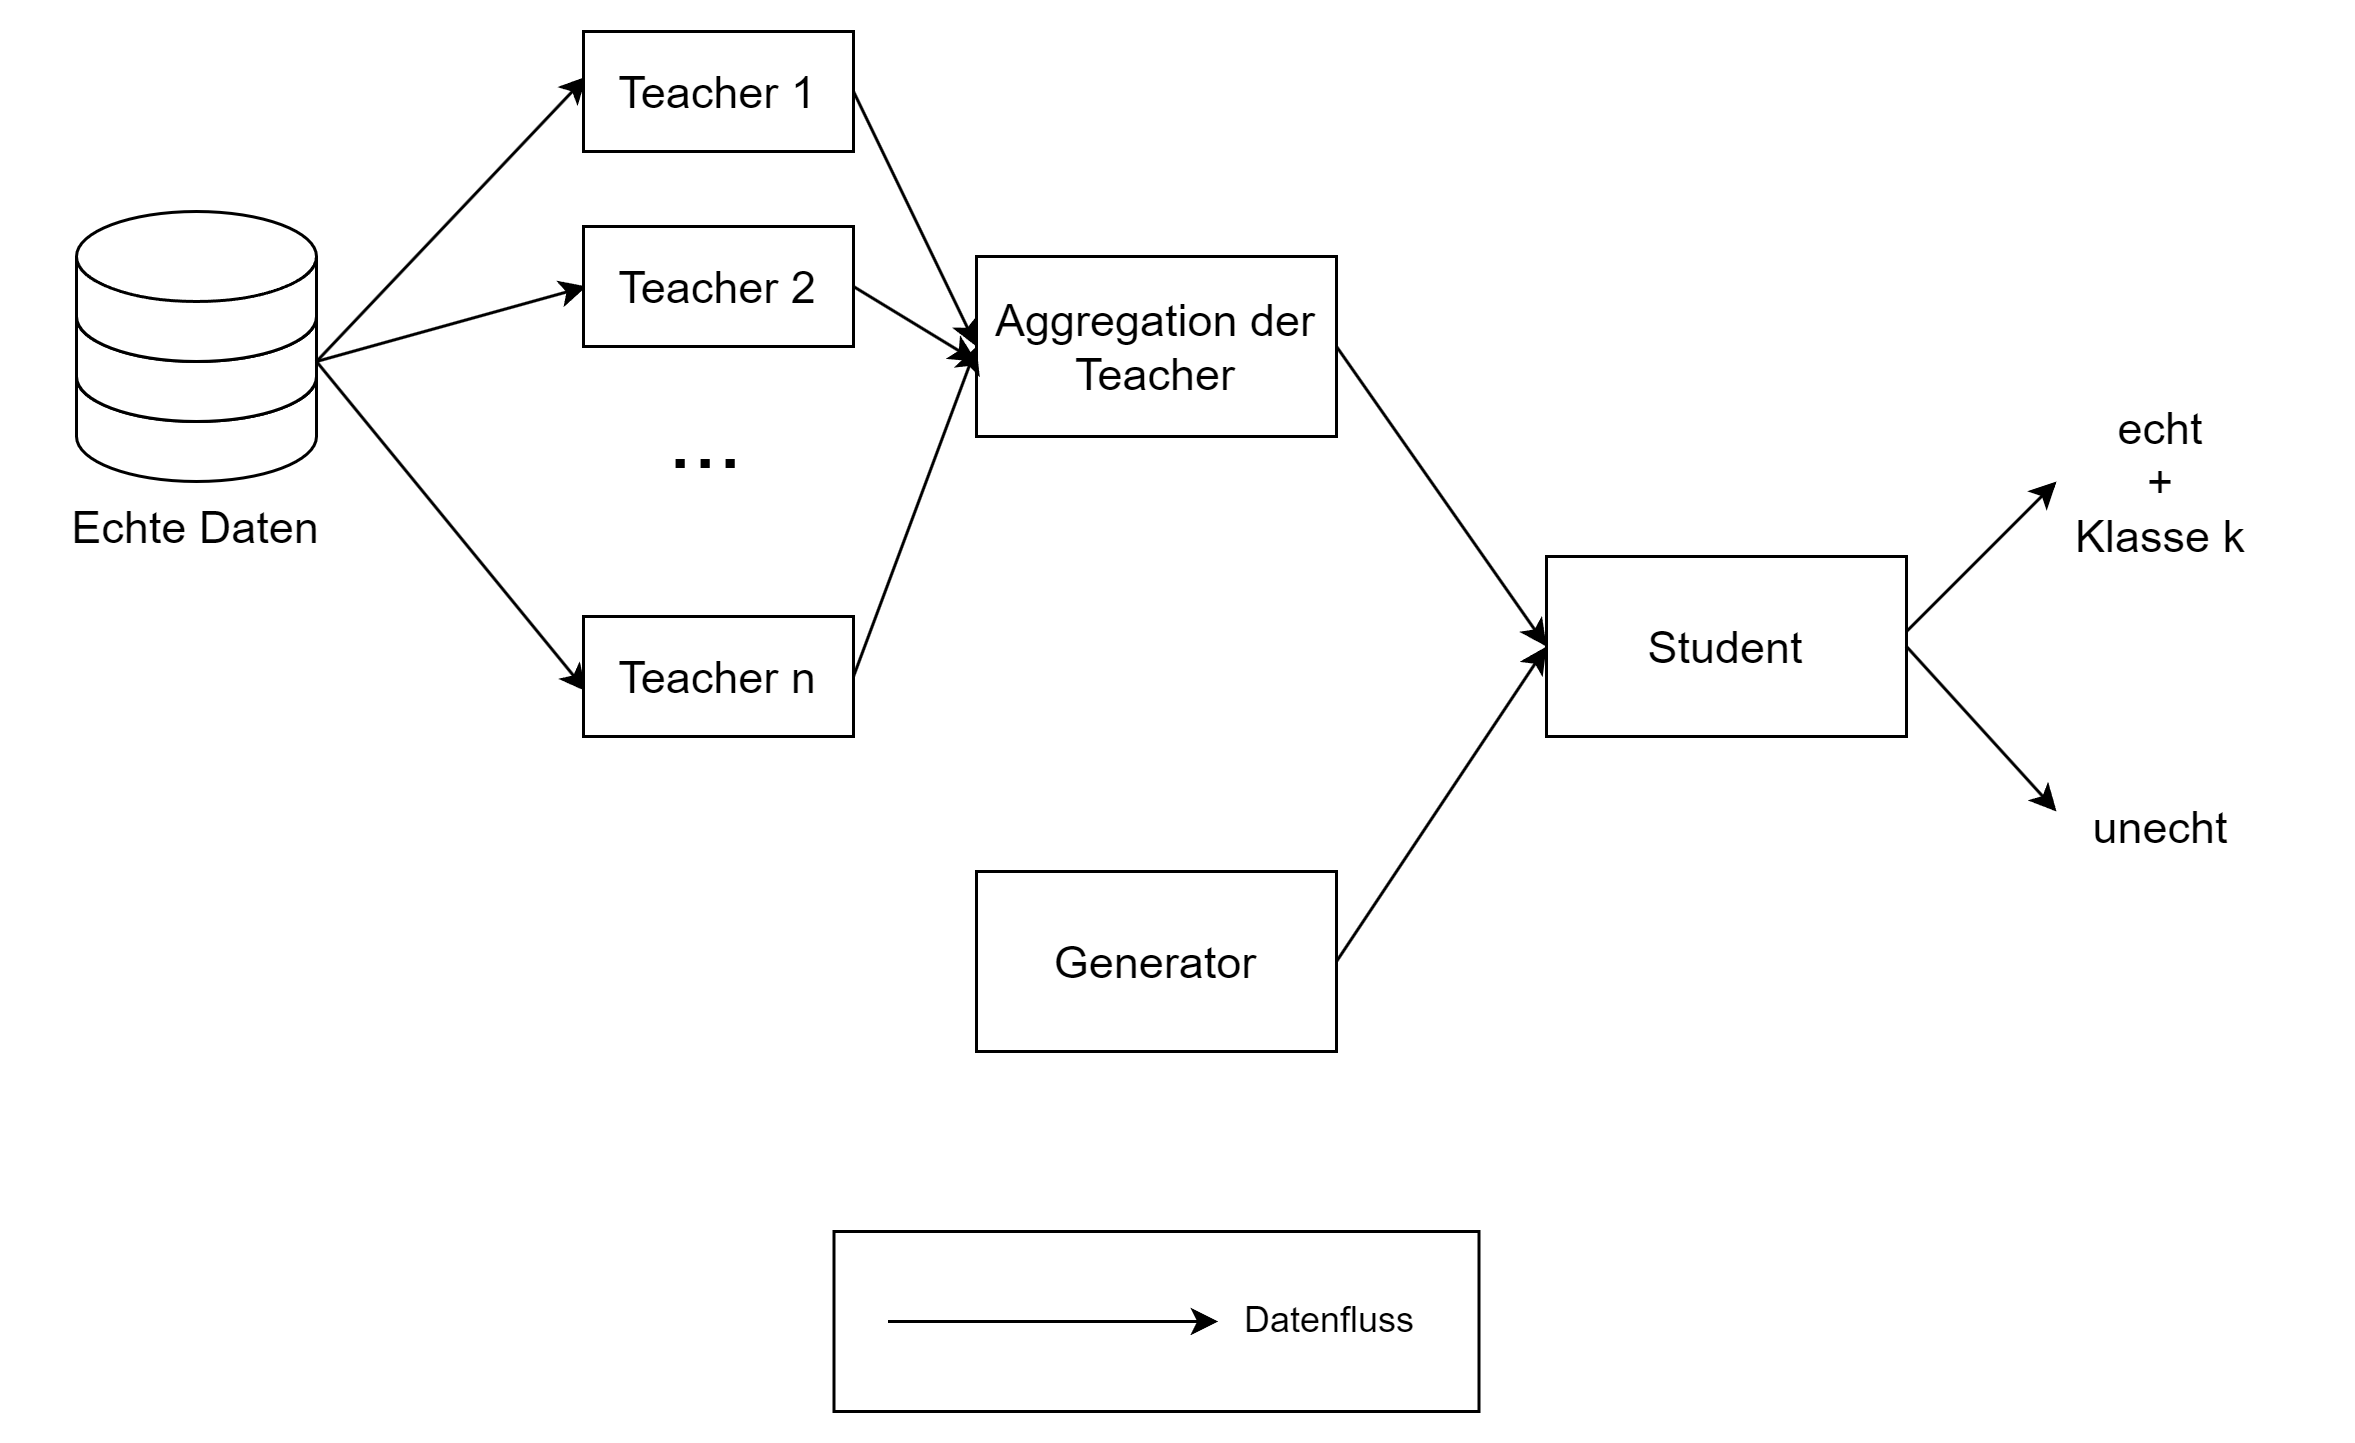
\includegraphics[width=15cm]{figures/pate_g.png}
    \caption{PATE-G}
    \label{fig:pate_g}
\end{figure} 

Die Autoren untersuchen zusätzlich noch mehrere Möglichkeiten, das Student-Modell zu trainieren  \cite{P-57}.
Die erfolgreichste Methode war ein teilweise beaufsichtigtes (semi-supervised) Lernen, welches auf GANs basiert.
Diese wird folglich PATE-G genannt.
Hier werden auch öffentliche, unsensible und ungelabelte Daten genutzt.
Teilweise werden die ungelabelten Daten mit der Aggregation der Teacher-Modelle gelabelt, dies ist jedoch nicht für alle Datenpunkte notwendig.
PATE-G nutzt den Student als Diskriminator eines GANs, der eine Klasse für \dq \textit{unechte Daten}\dq besitzt. 
Anstelle einer Klasse für \dq \textit{echte Daten}\dq, gibt es jedoch Neuronen für jede Klasse des Datensatzes.
Somit ist das Student-Modell ein Diskrimator, welcher jede echte Klasse klassifizieren kann, sowie zusätzlich eine Klasse für \dq \textit{unechte Daten}\dq besitzt.
Der Generator ist ein zusätzliches Neuronales Netz, welches Datensätze erzeugt, die versuchen, echten Datensätze nachzubilden.
Das Student-Modell, der Diskriminator, soll während des Trainings falsche Verteilungen in die Klasse für unechte Daten einordnen.
Echte, von den Teacher-Modellen gelabelte Daten, sollen der richtigen Klasse zugeordnet werden, wohingegen echte, ungelabelte Daten irgendeiner beliebigen, echten Klasse zugeordnet werden können.
Ein Vorteil von PATE-G ist, dass die ungelabelten Daten nicht verrauscht werden und sich dadurch das Privacy Budget nicht erhöht.
Obwohl die Klassen in dem Training des Student-Modells nicht zwingend richtig klassifiziert werden müssen, steigert dies dennoch die Güte des Modells.
Abbildung \ref{fig:pate_g} zeigt die bereits beschriebene Trainingsarchitektur von PATE-G.






